\section{Demonstration Problems}
% ============================= 
\subsection{Vortex induced vibration}
Vortex induced vibrations (VIV) are motions of solid structures immersed in fluid that is caused by the irregularities in the flow. VIV of structures is of practical interest to many fields of engineering. For example, it can cause vibration and noise in heat exchanger tubes and aircraft wing. The practical significance of VIV has led to various studies that are discussed in the literature\cite{williamson2004vortex}. In this demonstration problem, we are interested in the forced oscillations of an elastically mounted rigid cylinder for different values of the Reynolds number. The physical problem is shown in Figure \ref{fig:C5_cylinderShape}.
%
\begin{figure}[H]
    \centering
    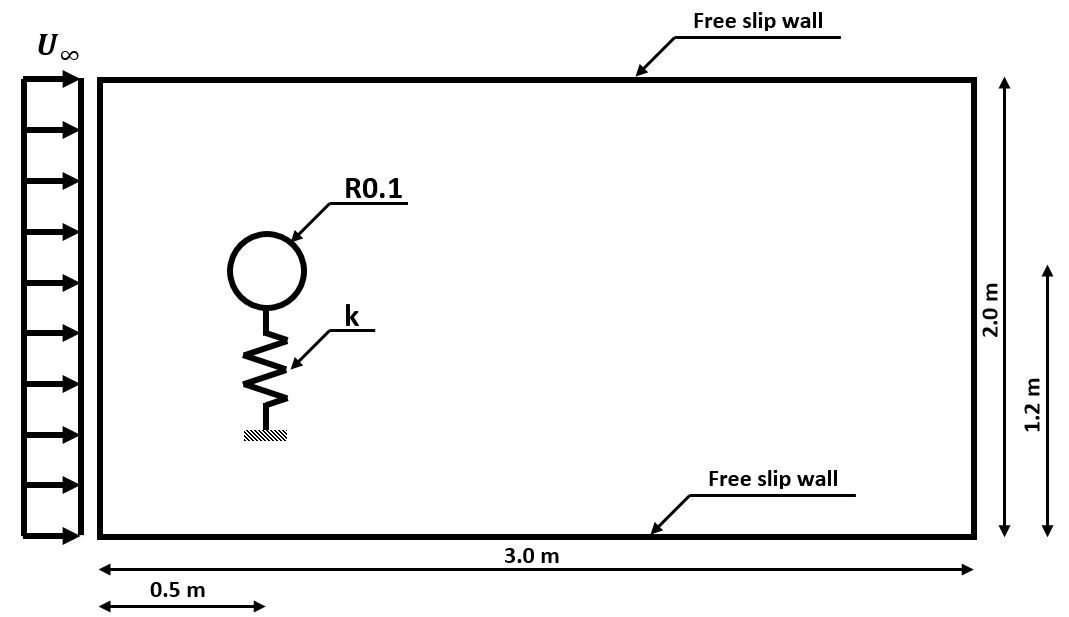
\includegraphics[width=9.00cm]{Chapter_5/figure/VIV_domain_shape.jpg}
    \caption{Physical domain for the vortex induced vibration problem.}
    \label{fig:C5_cylinderShape}
\end{figure}
%
The rigid cylinder has the radius of $R$ and mounted on an elastic structure with stiffness $k$. The free steam velocity is selected as $U_\infty$. To verify the solver and FSI coupling, we are going to calculate the shedding frequency of the cylinder first. Vortex shedding is an oscillating flow that takes place when fluid passes a bluff body at certain velocities. The vortices that are generated on the aft of the body start to detach periodically from either side of the body. The frequency at which the vortex shedding takes place is described using the dimensionless Strouhal number. The Strouhal number is defined as shown in Equation \eqref{eq:C5_strouhalNumber}.
%
\begin{equation}\label{eq:C5_strouhalNumber}
	St = \frac{fL}{U}
\end{equation}
%
where $f$ is the frequency of the vortex shedding, $L$ is the characteristic length, and $U$ is the flow velocity. The Strouhal number of a stationary circular cylinder is a function of Reynolds number \cite{chen1987flow} as shown in Figure \ref{fig:C5_strouhalVSreynoldsNumber}.
%
\begin{figure}[H]
    \centering
    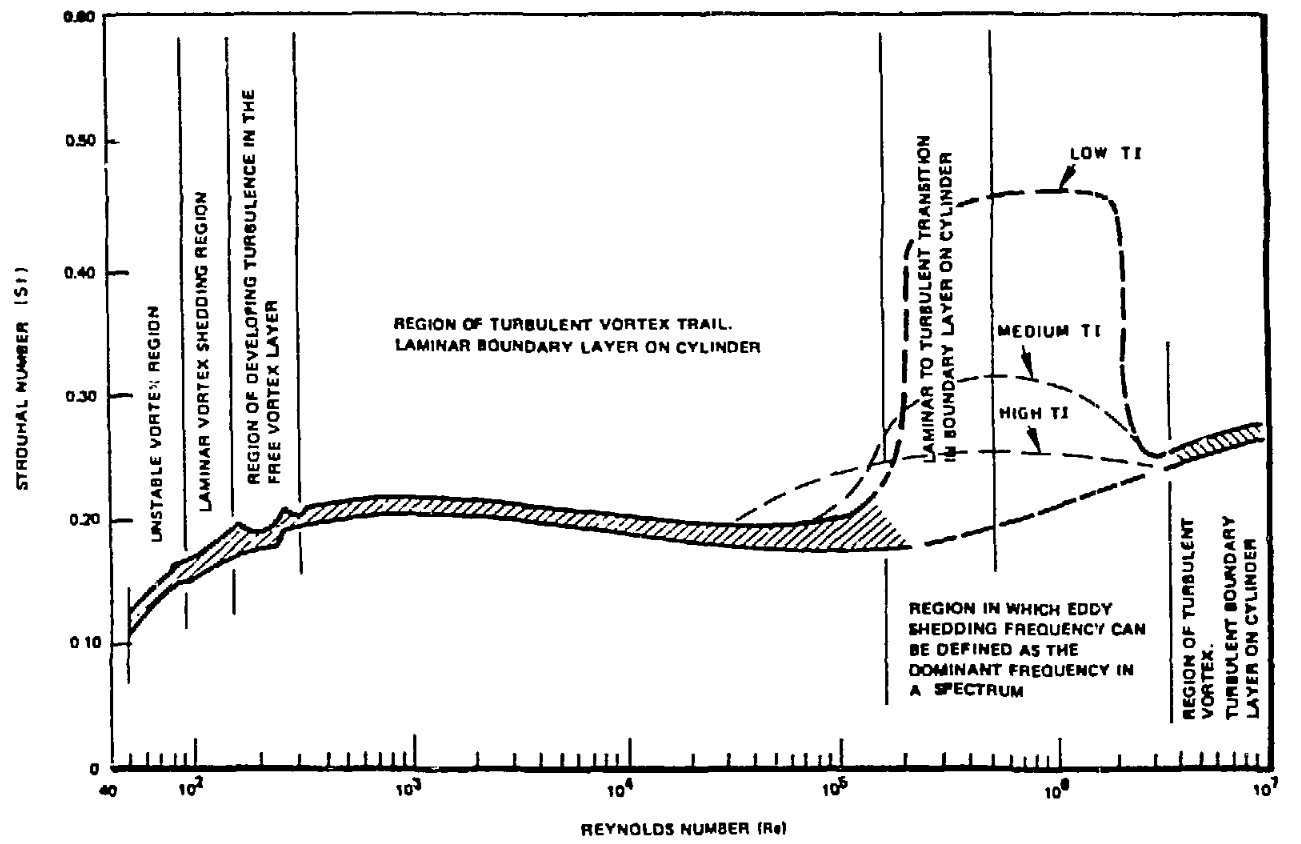
\includegraphics[width=10.00cm]{Chapter_5/figure/StrouhalVsReynodsl.png}
    \caption{PStrouhal number for a single cylinder\cite{jendrzejczyk1985fluid}.}
    \label{fig:C5_strouhalVSreynoldsNumber}
\end{figure}
%
To verify the simulation code developed for the IB simulation, we verified the shedding frequency of the circular cylinder in the cross-flow using Equation \eqref{eq:C5_strouhalEquationForCylinder}. The domain length and height are selected as $3 m$ and $2 m$ respectively as shown in Figure \ref{fig:C5_cylinderShape}. The cylinder radius is selected as $0.1 m$ and is located $0.5 m$ from the left wall and $1.2 m$ from the bottom wall. The assymetric shape of the computational domain helps the shedding initiation. The domain is discretized using $3000$ cells in the $x$ and $2000$ in the $y$ direction. The cylinder is defined using $50$ Lagrangian nodes. The $p$ value in the delta function definition is selected as $0.5$. It should be noted that to verify the shedding frequency the cylinder is fixed in its place. We compared the Strouhal number calculated from the IB code with the results \cite{mittal2001control} for two different Reynolds numbers. The shedding frequency is calculated by saving the time history of drag force on the cylinder and performing frequency analysis on this data. We used the power spectral density function to look at the most dominant frequencies. The comparison between these results are shown in Table \ref{table:C5_strouhalVerification}.
%
\begin{table}[H]
\centering
\begin{tabular}{c | c | c}
     Reynolds number & St (current IB) & St (Literature \cite{mittal2001control} and \cite{jendrzejczyk1985fluid}) \\ \hline \hline
     100 & 0.170 & 0.168 \\ \hline
     500 & 0.194 & 0.200 \\
\end{tabular}
\caption{Comparison between the shedding frequency calcualted using IB method and results from the literature.}
\label{table:C5_strouhalVerification}
\end{table}
%
The effect of number of Lagrangian points on the shedding frequency is shown in Figure \ref{fig:C5_numberOfLagrangianOnSheddingFreq} for the two Reynolds numbers of 100 and 500.